\documentclass[11pt, oneside]{article} 
\usepackage{geometry}
\geometry{letterpaper} 
\usepackage{graphicx}
	
\usepackage{amssymb}
\usepackage{amsmath}
\usepackage{parskip}
\usepackage{color}
\usepackage{hyperref}

\graphicspath{{/Users/telliott/Github/precalculus/fig/}}
% \begin{center} \includegraphics [scale=0.4] {gauss3.png} \end{center}

\title{Simple slopes}
\date{}

\begin{document}
\maketitle
\Large

\label{sec:slopes}

\hypertarget{first_calculus}{}

To introduce the two fundamental ideas in calculus, consider two measuring devices used while driving a car.  Most good drivers look fairly often at the speedometer, which measures speed or velocity, or how fast you're going.  

On the other hand, if someone gives you directions like --- go three and a half miles and then turn left (where the old gas station used to be), you need to be watching your odometer.

\begin{center} 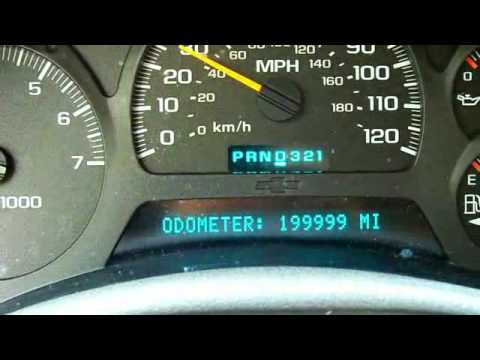
\includegraphics [scale=0.4] {hqdefault.jpg} \end{center}

Distance divided by time is velocity.  Velocity times time equals distance.  We can think of speed and velocity as the same for now.

Velocity is the \emph{rate of change} of distance with time, it has units like miles per hour or feet per second (15 mph is exactly 22 feet per second;  $15 \cdot 5280 = 22 \cdot 3600$).

In calculus we say that

$\circ$ \ velocity is the \textbf{derivative} of the distance with respect to time

$\circ$ \  distance is the \textbf{integral} of the velocity with respect to time

We can speak of velocity at a particular time $t$, as in "our current velocity is 60 miles per hour."  But the distance, the integral, must be evaluated between appropriate starting and stopping points for the time.

In our example, you must first look at your odometer \emph{before} you start on that $3.5$ mile drive, and subtract the initial from the final value.

\subsection*{time-dependence}
Distance equals velocity times time.

This is easy if the velocity is constant.  Travel west on the interstate at exactly $60$ miles per hour for $2$ hours and your distance will be $120$ miles from where you started (provided you don't start in Los Angeles).  

It is standard to use $s$ to refer to the distance traveled and $v$ for velocity.  If the velocity is constant then:
\[ s = vt \]
According to the internet, $s$ is from the Latin "spatium", for "space, room, or distance."

Suppose we plot velocity as a \emph{function of time} with $v$ on the $y$-axis and $t$ on the $x$-axis.

\begin{center} 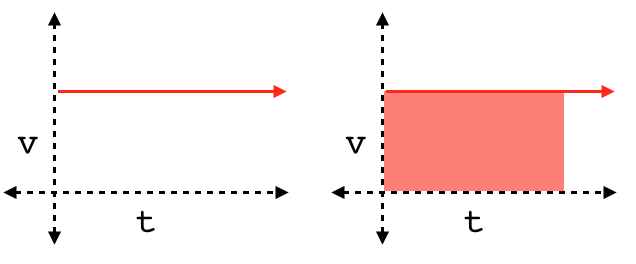
\includegraphics [scale=0.5] {velocity_time_3.png} \end{center}

Since the velocity is constant, the result is a straight horizontal line.  

Furthermore, the distance traveled is the \emph{area under the curve} (and above the $x$-axis) which is the area of a rectangle with sides $v$ and $t$ and as we said 
\[ s = vt \]

However, for most interesting problems the velocity is not constant.  

Imagine maintaining pressure on the gas pedal in the car steadily so that, starting from a stop at zero time, after $1$ second your velocity is $10$ mph, after $2$ seconds it is $20$ mph, after $3$ seconds, $30$ mph. If we continue at the same rate of acceleration, we'll go from $0$ to $60$ mph in $6$ seconds, which is quite a respectable time.

This example has constant acceleration.  Here, we say that $v$ is a constant function of time, and write 
\[ v = at \]
where $a$ is the acceleration.

\begin{center} 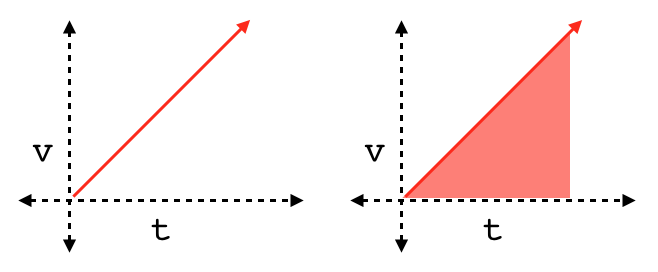
\includegraphics [scale=0.5] {velocity_time_4.png} \end{center}
What about the distance?  It turns out that the distance is once again the area under the curve.

Since $a$ isn't zero, $v$ must change with time.  

If $a$ is non-zero and constant, then $v$ changes at a constant rate.  Starting from $0$, the final velocity will be $v = at$, but the distance traveled is no longer the product 
\[ s = v \times t \stackrel{?}{=}  \]

because this $v$ is the final velocity and that is not the correct $v$ to use.  For variable velocity, the distance traveled is the \emph{average} velocity times the time.  For smooth (constant) acceleration from zero to $v$, the average velocity is the average of the initial and final velocities:
\[ v_{\text{avg}} = \frac{1}{2} \ (v_i + v_f) = \frac{1}{2} \ v \]

So the correct equation is:
\[ s = v_{\text{avg}}\ t  = \frac{1}{2} \ v \cdot t \]
and since $v = at$
\[ s = \frac{1}{2} at^2 \]

In this case, if we plot velocity as a function of time, we obtain a straight line that extends diagonally up with respect to the $x$-axis.  The distance traveled is the area under the curve, below the line and above the $x$-axis.  

The shape whose area is needed is a triangle.  This also accounts for the factor of $1/2$.

\begin{center} 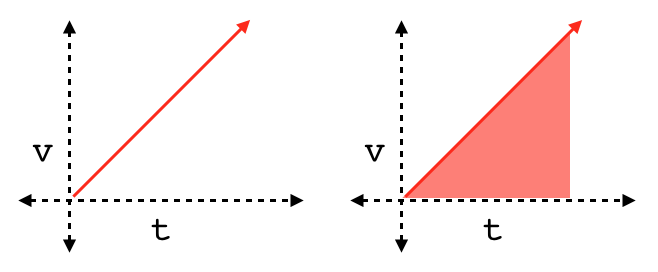
\includegraphics [scale=0.5] {velocity_time_4.png} \end{center}

You probably know that if a mass $m$ is dropped from a tall building like the Tower of Pisa, then the distance it has fallen goes like the square of the time.  The equation is:
\[ s = \frac{1}{2} g t^2 \]
where $g$ is the acceleration due to gravity.

Notice that this is the same equation as we just obtained.

The reason is that $g$ is approximately constant near the surface of the earth, its value is about $10$ in units of m/s$^2$.  A fall of four seconds is about 80 meters.

Galileo knew this formula (at least, he knew the $t^2$ part of it), which he obtained not from experiments at the Tower of Pisa, but by timing the descent of balls down an inclined plane.

\begin{center} 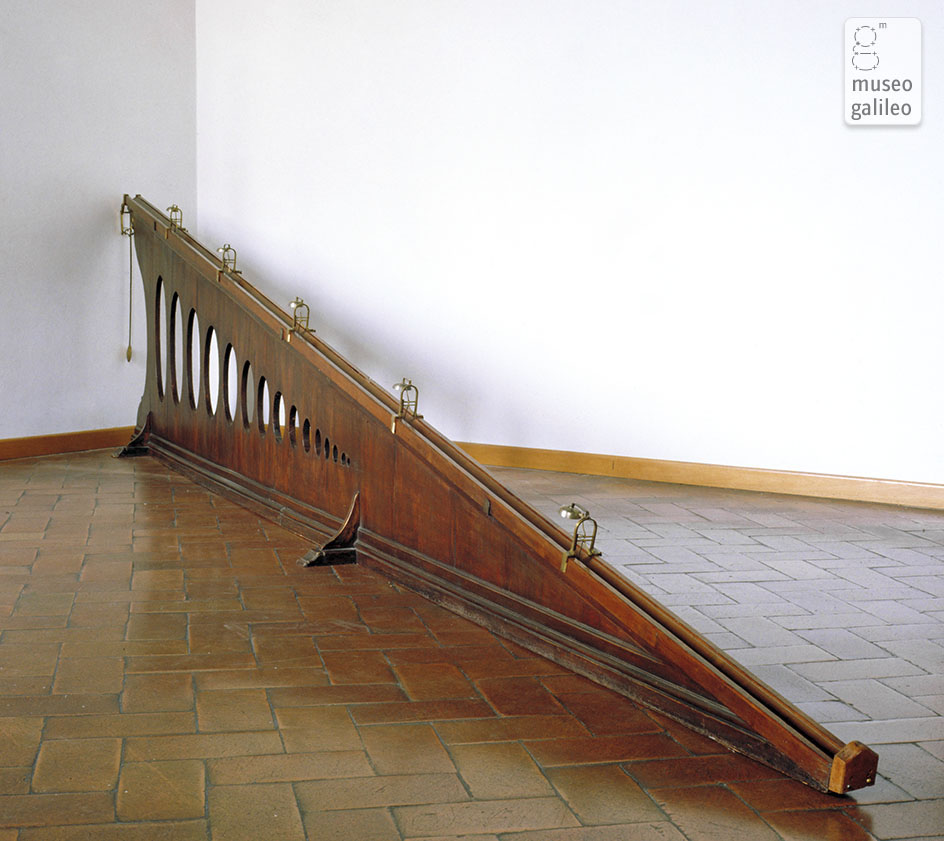
\includegraphics [scale=1.25] {galileo_plane.jpg} \end{center}

\subsection*{initial position and velocity}

If you want to be more complete and say that the starting point is not necessarily the origin of the coordinate system, add a constant $s_0$ to describe the initial distance from the origin and obtain:
\[ s = vt + s_0 \]
and similarly, a constant $v_0$ to describe the initial velocity as shown above.

The full equation of motion is 
\[ s = \frac{1}{2} a t^2 + v_0 t + s_0 \]

We'll say much more about this later.

\subsection*{power rule}

We will introduce the theory of calculus more formally in the next section of the book.  For now, we just talk about a simple rule called the power rule.

Switching notation to $y$ and $x$, suppose that $y$ is a \emph{function} of $x$ and write $y = f(x)$.

Here are three types of dependency (with $c$ as a constant), with three corresponding types of graph.

$\circ$ \ $y = c$

$\circ$ \ $y = cx$

$\circ$ \ $y = cx^2$

These are (respectively) the equations of:  (i) a horizontal line, since $y$ is constant, (ii) any other non-vertical line ($y$ is proportional to $x$), and (iii), a parabola.

\begin{center} 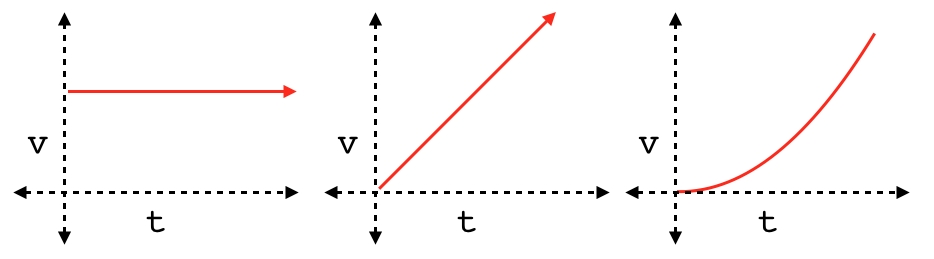
\includegraphics [scale=0.4] {functions.png} \end{center}

Suppose we are at some particular point on the curve, $x$.

We ask "what happens if we change $x$ a little bit" and use the notation $dx$ to refer to this little bit of $x$.  

What happens to $y$?  $y$ will usually change by a small amount.  Call that amount $dy$.

\subsection*{case 0}
We can call this case 0 because we can write it as
\[ y = cx^0 = c \]

Of course, in this case 
\[ y = c \]
$y$ does not actually depend on $x$ at all.  The change $dy$ resulting from a change in $x$, $dx$, is zero.  That is what the curve plotted above tells us (left panel).
\[ y = c, \ \ \ \ dy = 0 \cdot dx \]

The ratio $dy/dx$ is the slope of the curve formed by plotting $y$ against $x$.  We call that slope the \emph{derivative} of the function $f(x)$.

Divide both sides by $dx$ and rewrite the above as:
\[ \frac{dy}{dx} = 0 \]

This plot is a horizontal line with slope $0$.

\subsection*{case 1}
Here, $y$ is a linear function of $x$, the change $dy$ is the change $dx$ multiplied by $c$:
\[ y = cx, \ \ \ \  dy = c \cdot dx \]
rearranging.
\[ \frac{dy}{dx} = c \]

In analytical geometry, we calculate the slope of a line as $\Delta y/\Delta x$.

For a line, the slope is constant and so it doesn't matter which two points with coordinates $(x,y), (x',y')$ we choose for the calculation.  The following is true for \emph{any} two points on the line:
\[ m = \frac{\Delta y}{\Delta x} = \frac{y - y'}{x - x'} \]

Above we had the example where $v = at$ with constant $a$.  Then $dv/dt = a$.

\subsection*{case 2}
This case is different.
\[ y = cx^2 \]

We finally get to using some calculus.

For a parabola, the slope of the curve at a point (the slope of the tangent to the curve $y = cx^2$) depends on the choice of $x$.  The slope is steeper the further out you go in a positive direction on the $x$-axis (right panel).

\begin{center} 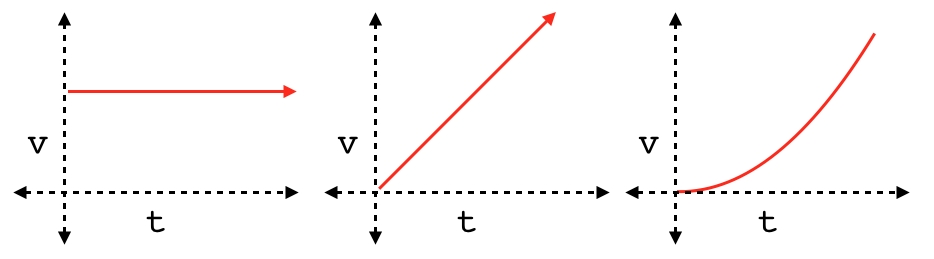
\includegraphics [scale=0.4] {functions.png} \end{center}

It seems impossible to compute the slope of this curve in the standard way, by picking two points $(x,y)$ and $(x',y')$ and then calculating $\Delta y/\Delta x$, because the slope changes as we go out along the curve.  You'll get a different answer for each different $x$.

\subsection*{key idea}

The insight is that if $x$ is sufficiently close to $x'$ the slope is approximately constant.  It's like saying that the earth is flat \emph{locally}.  If you detect any curvature, just zoom in a bit.  In the figure below

\begin{center} 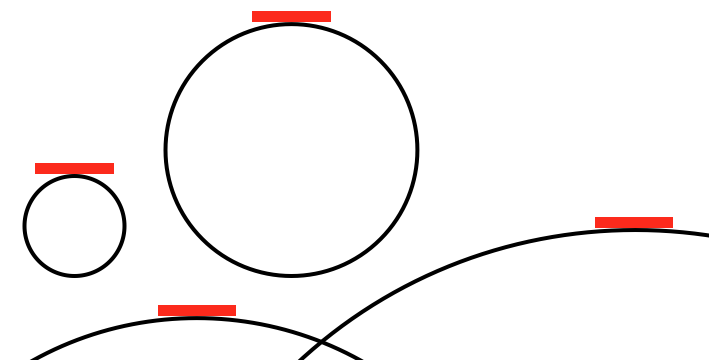
\includegraphics [scale=0.5] {line_circles.png} \end{center}

the distance to the circle from the end of a line of fixed length decreases as we increase the size of the circle.

In calculus, we don't make the curves larger, we make the distance between $x$ and $x'$ smaller and smaller until it is so small, that the circle, or the parabola in the other figure, becomes flat.  I have just magnified the figure so we could see it.

The error, the distance between the end of the red line above and the circle, gets smaller and smaller as a fraction of the line's length.  Our approximation gets better and better.  Just zoom in until the line is a good enough approximation to the shape of the circle, if the curve doesn't look flat enough, zoom in some more.

As we are accelerating in the car, with constantly changing velocity, we can still have a unique velocity at a particular instant in time.

In mathematical language, for a very small change $\Delta x$ in either direction from $x$, we get the same slope, \emph{if} $\Delta x$ is small enough. 

If it's not, we can always make it smaller.  That's the beauty of the real numbers.

As you accelerate from 0 to 60, there must be at least one moment in time when your velocity is 50. 

Or, put still another way, when they built your house they didn't worry about the curvature of the earth.

If $r$ is the radius of the earth in feet, and the house is $a = 50$ feet long, the drop due to curvature is $r - b$ where $b = \sqrt{r^2 - l^2}$

\begin{verbatim}
r = 21120000
b = 21119999.9999408
\end{verbatim}

That is about $0.00006$ feet over the length of a $50$ foot house, about a thousand times less than $1/16$ of an inch.  It is nearly 6 orders of magnitude, one part in a million.

Since the changes in $x$ and $y$ are so small, we use the new nomenclature:  $dy$ and $dx$.

\subsection*{power rule}
To actually calculate slopes for curves (and straight lines), use the power rule.

For a horizontal line with zero slope:
\[ y = c \]
\[ \frac{dy}{dx} = 0 \]

For a line with a slope $c$:
\[ y = cx \]
\[ \frac{dy}{dx} = c \]

For the parabola, the rule says that if $y = cx^2$, the slope or derivative is
\[ \frac{dy}{dx} = 2cx \]

We've been writing $c$ as the constant, so as not to confuse it with $a$, the acceleration.  In analytic geometry, a parabola is usually written with a constant $a$, called the shape factor:
\[ y = ax^2 \]
Then, the slope is $2ax$.  

If we had
\[ y = ax^2 + bx + c \]
with $a,b,c$ all constant, then the slope would be $2ax + b$.  

The above uses our three rules from above, plus one more, that when taking the derivative of a polynomial, the derivative of the whole is simply the summed derivatives for each term.

For the equation of motion under gravity
\[ s = \frac{1}{2} a t^2 + v_0 t + s_0 \]
\[ v = \frac{ds}{dt} = at + v_0 \]
\[ \frac{dv}{dt} = a \]
Notice how the $1/2$ and the $2$ cancel in the second equation.

Continuing to the cubic, if $y$ depends on $x^3$ like
\[ y = cx^3 \]
then
\[ \frac{dy}{dx} = 3cx^2 \]

The general form of the power rule is that if
\[ y = x^n \]
then
\[ \frac{dy}{dx} = n x^{n-1} \]

The exponent has been reduced by $1$ power, and the value of that exponent applied as a factor in front of the expression.

This rule had already been discovered before Newton.  It's a toss-up whether Fermat or Cavalieri was first.  We will prove this later, but for now we just want to introduce the idea and practice using it.

\subsection*{note}
If you already know some calculus you're probably jumping out of your chair while reading this chapter because you've had it pounded into you that $dy/dx$ is not a quotient and believe that you can't simply multiply both sides of the equation by $dx$.

Well, you can.  And I'll explain why as we go along.

\end{document}